\documentclass{beamer}

\usetheme{Boadilla}

\newcommand{\bi}{\begin{itemize}}
\newcommand{\ei}{\end{itemize}}
\newcommand{\I}{\item}
\newcommand{\f}{\frame}
\newcommand{\ft}{\frametitle}

\title{Introduction and Overview}
\subtitle{for the FDC-Mini Review}
\author[M.\ Ito]{Mark M.\ Ito}
\date{February 1, 2008}
\institute[JLab]{Jefferson Lab}

\begin{document}

\f{\titlepage}

\f{
  \ft{Outline}
  \bi
  \I physics goals
  \I history: previous reviews
  \I general design considerations
  \I backgrounds
  \I specifications
  \I resolution estimates
  \I conclusions
  \ei
}

\f{
  \centerline{\Large physics goals}
}
\f{
  \ft{goals and requuirements}

The search for exotic mesons is at a turning point. The experiments at
BNL, Protvino, and at LEAR which have reported evidence for exotic
mesons have terminated data taking; data analysis is completed...new
experiments are ahead of us, COMPASS at CERN and BESIII in the
immediate future, the Hall-D experiment at the upgraded JLab
facility and PANDA at GSI in the medium-range future. --- Eberhard
Klempt

  \bi
  \I Map the spectrum of hybrid mesons (gluonic excitations)
    \bi
    \I Start with those with exotic quantum numbers
    \I Make contact with spectroscopy of non-exotic states
    \ei

  \I Analysis will require
    \bi
    \I partial-wave analysis
    \I identification of exclusive final states
    \I detailed understanding of backgrounds
    \I large event samples
    \I confirmation of states in multiple decay channels
    \ei
  \ei
}
\f{
  \ft{lattice mass predictions}
  Lowest mass expected to be $\pi_1(1^{−+})$ at $1.9 \pm 0.2$~GeV
$$
  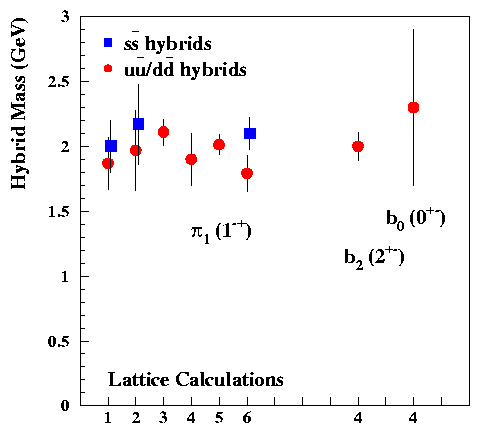
\includegraphics[height=3in]{hybrids_lattice.png}
$$
}
\f{
  \ft{representative kinematics}
$$
  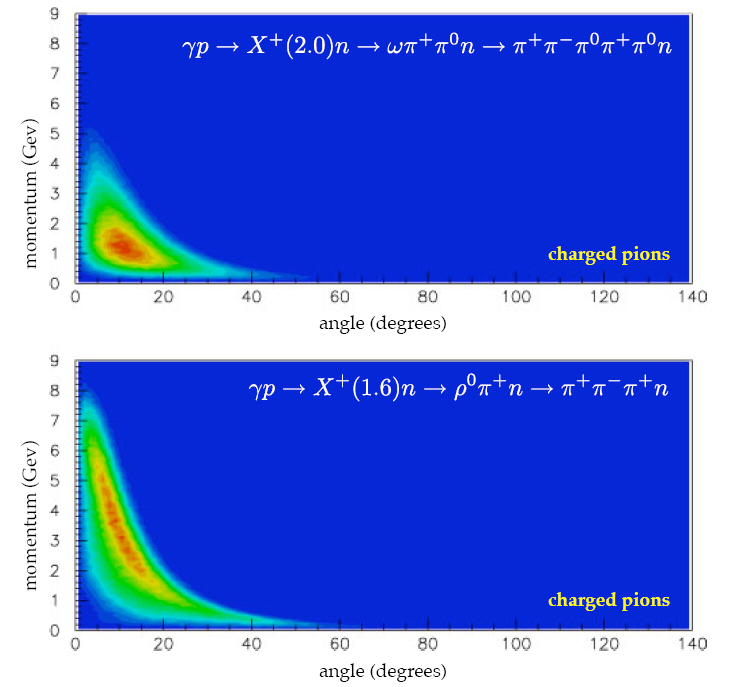
\includegraphics[height=3in]{kinematics.png}
$$
}
\f{
  \ft{anything else?}
  \bi
  \I Hall D a unique facility
    \bi
    \I high-energy tagged photon beam
    \I coherent bremsstrahlung $\Rightarrow$ nearly mono-energetic beam
    \I linear polarization
    \ei
  \I driven to a general purpose detector
    \bi
    \I charged and neutral particle detection
    \I very large acceptance
    \ei
  \I other physics possible!
    \bi
    \I come to the workshop, PHP2008, March 6-8, at JLab
    \I ``Photon-hadron physics with the GlueX detector at Jefferson Lab''
    \ei
  \ei
}
\f{
  \centerline{\Large reviews, past and future}
}
\f{
  \centerline{\Large general design considerations}
}
\f{
  \centerline{\Large backgrounds}
}
\f{
  \centerline{\Large specifications}
}
\f{
  \centerline{\Large resolution estimates}
}
\f{
  \centerline{\Large conclusions}
}

\f{
\ft{leftovers}
cd3 in june
dc review in march
why this charge
momentum and angle range
dc review last march
recommendations
position resolution
dominated by multiple scattering
material reduction
wires-only
nominal 2 cathode-readout layers per anode layer design
savings in electronics
pipeline data-acquisition
fadc readout combines time and charge
dedx possible
cost savings
with cathode and anode read-out: disambiguate using timing
  possible to get 3-d points in a single tracking layer
time resolution
no segmentation in azimuth
  cdc
  clas
  tpc
narrow resonances: good resolution reduced background
kinematic coverage
required momentum resolution
smooth acceptance
well-understood acceptance
large acceptance
robust pattern recognition
full court press
backgrounds
  electronic noise
  e\&m
  hadronic
  combinatoric
}

\end{document}

%%% end of latex file %%%%
